\documentclass[12pt,a4paper]{article}

% Required packages
\usepackage[utf8]{inputenc}
\usepackage[T1]{fontenc}
\usepackage{geometry}
\usepackage{graphicx}
\usepackage{booktabs}
\usepackage{hyperref}
\usepackage{enumitem}
\usepackage{tikz}
\usetikzlibrary{shapes.geometric, arrows, positioning}

% Page geometry
\geometry{top=1in, bottom=1in, left=1in, right=1in}

% Flowchart styles
\tikzstyle{startstop} = [rectangle, rounded corners, minimum width=3cm, minimum height=1cm,text centered, draw=black, fill=white]
\tikzstyle{process} = [rectangle, minimum width=3cm, minimum height=1cm, text centered, draw=black, fill=white]
\tikzstyle{decision} = [diamond, minimum width=3cm, minimum height=1cm, text centered, draw=black, fill=white]
\tikzstyle{arrow} = [thick,->,>=stealth]

\begin{document}

% Title Page
\begin{titlepage}
    \centering
    \scshape
    \vspace*{1cm}
    {\huge\bfseries Project Proposal \& System Design\par}
    \vspace{0.5cm}
    {\Large Smart Gate Management System\par}
    \vspace{1.5cm}
    {\large Academic Semester Project: Software Engineering\par}
    \vspace{2cm}
    
    \begin{table}[h]
        \centering
        \begin{tabular}{ll}
            \textbf{Lead Developer:} & Pratibha \\
            \textbf{Date:} & March 11, 2026 \\
            \textbf{Methodology:} & Agile Scrum
        \end{tabular}
    \end{table}

    \vfill
    {\large \today\par}
\end{titlepage}

\tableofcontents
\newpage

\section{Problem Statement}
Manual visitor logbooks at gated communities and offices are inefficient, insecure, and prone to data theft. Existing issues include:
\begin{itemize}
    \item \textbf{Identity Fraud}: Anyone can write a fake name or phone number.
    \item \textbf{Slow Processing}: Visitors wait for minutes while guards manually record data.
    \item \textbf{No Host Notification}: Residents are often unaware of a visitor's arrival until they are at the door.
    \item \textbf{Data Inaccessibility}: Searching for a specific entry in a physical book is nearly impossible.
\end{itemize}

\section{Proposed Approach}
We propose a web-based \textbf{Smart Gate System (SGS)} using a 2-Phase Agile approach:
\begin{enumerate}
    \item \textbf{Digital Verification}: Replace signatures with OTP (One-Time Password) verification via Email/SMS.
    \item \textbf{Instant Notification}: Automated alerts to the host person.
    \item \textbf{QR-Based Access}: Once verified, visitors receive a temporary QR code for faster gate interaction.
\end{enumerate}

\section{Proposed Solution}
The solution is a distributed full-stack application:
\begin{itemize}
    \item \textbf{Backend}: Node.js and Express processing identity validation logic.
    \item \textbf{Database}: MongoDB storing visitor logs, blacklists, and host records.
    \item \textbf{Security}: JWT tokens for Guard/Admin logins and Bcrypt for data hashing.
\end{itemize}

\section{System Functionality}
\subsection{Visitor Module}
\begin{itemize}
    \item Self-registration via a unique mobile link.
    \item OTP-based mobile number verification.
    \item Auto-generation of Visitor Pass after verification.
\end{itemize}

\subsection{Security Guard Dashboard}
\begin{itemize}
    \item Real-time visitor log monitoring.
    \item Blacklist checking system.
    \item Physical entry/exit timestamp recording.
\end{itemize}

\section{User Interface Design}
The UI is designed with a "Mobile-First" philosophy using clean HTML5/CSS3.
\begin{itemize}
    \item \textbf{Visitor View}: A minimalist, single-page form to minimize data entry time.
    \item \textbf{Guard Dashboard}: High-contrast, tabular view optimized for tablets.
    \item \textbf{Admin Panel}: Secure portal for managing blacklisted numbers and host directories.
\end{itemize}

\section{Project Timeline \& Responsibilities}
The project followed an Agile Scrum methodology over an 8-week period. The following table outlines the key tasks and the division of labor between the two team members.

\begin{table}[h]
    \centering
    \small
    \begin{tabular}{@{}llll@{}}
        \toprule
        \textbf{Task} & \textbf{Phase} & \textbf{Primary Owner} & \textbf{Status} \\ \midrule
        Requirements \& IEEE SRS & Phase 1 & Riya (QA/Doc) & Completed \\
        Architecture \& DB Design & Phase 1 & Pratibha (Dev) & Completed \\
        Backend API (Node/Express) & Phase 1 & Pratibha (Dev) & Completed \\
        Local OTP Logic & Phase 1 & Pratibha (Dev) & Completed \\
        Phase 1 Technical Report & Phase 1 & Riya (QA/Doc) & Completed \\ \midrule
        Firebase Auth Integration & Phase 2 & Pratibha (Dev) & Completed \\
        Testmail.app Gateway & Phase 2 & Pratibha (Dev) & In Progress \\
        QR Code Generation & Phase 2 & Pratibha (Dev) & In Progress \\
        Final LaTeX Report & Phase 2 & Riya (QA/Doc) & In Progress \\ \bottomrule
    \end{tabular}
    \caption{Project Execution Timeline and Task Allocation}
\end{table}

\section{System Architecture \& Workflow}

\subsection{Architectural Components}
The Smart Gate System is built using the \textbf{MERN-like stack} (MongoDB, Express, Node.js) with a focus on modularity and security.
\begin{enumerate}
    \item \textbf{Presentation Layer}: Developing using HTML5, CSS3, and JavaScript to ensure a responsive mobile-first experience for visitors and guards.
    \item \textbf{Application Layer}: A Node.js and Express.js server that handles the business logic, OTP generation, and visitor validation.
    \item \textbf{Data Layer}: MongoDB (Atlas) for persistent storage of visitor logs, host information, and blacklisted entities.
    \item \textbf{External Services}: Integration with \textbf{Testmail.app} for high-reliability OTP/E-Pass delivery and \textbf{Firebase} for secure authentication.
\end{enumerate}

\subsection{Operational Workflow}
The system operates through a structured sequence to ensure security at the gate:
\begin{itemize}
    \item \textbf{Step 1: Initiation}: The visitor scans a QR code at the gate or follows a registration link.
    \item \textbf{Step 2: Verification}: The system generates a 6-digit OTP and sends it to the visitor via \textbf{Testmail.app} (Automated Email Service). The visitor must enter this code to prove their identity.
    \item \textbf{Step 3: Security Check}: The system automatically checks the visitor's phone number against the global \textbf{Blacklist}.
    \item \textbf{Step 4: Approval}: If valid, the host is notified, and a digital visitor pass (QR Code) is generated and emailed to the visitor for the Security Guard to scan.
\end{itemize}

\subsection{End-to-End Data Flow}
The following diagram illustrates the complete data lifecycle, from the initial visitor request to the final gate entry authorization:

\begin{center}
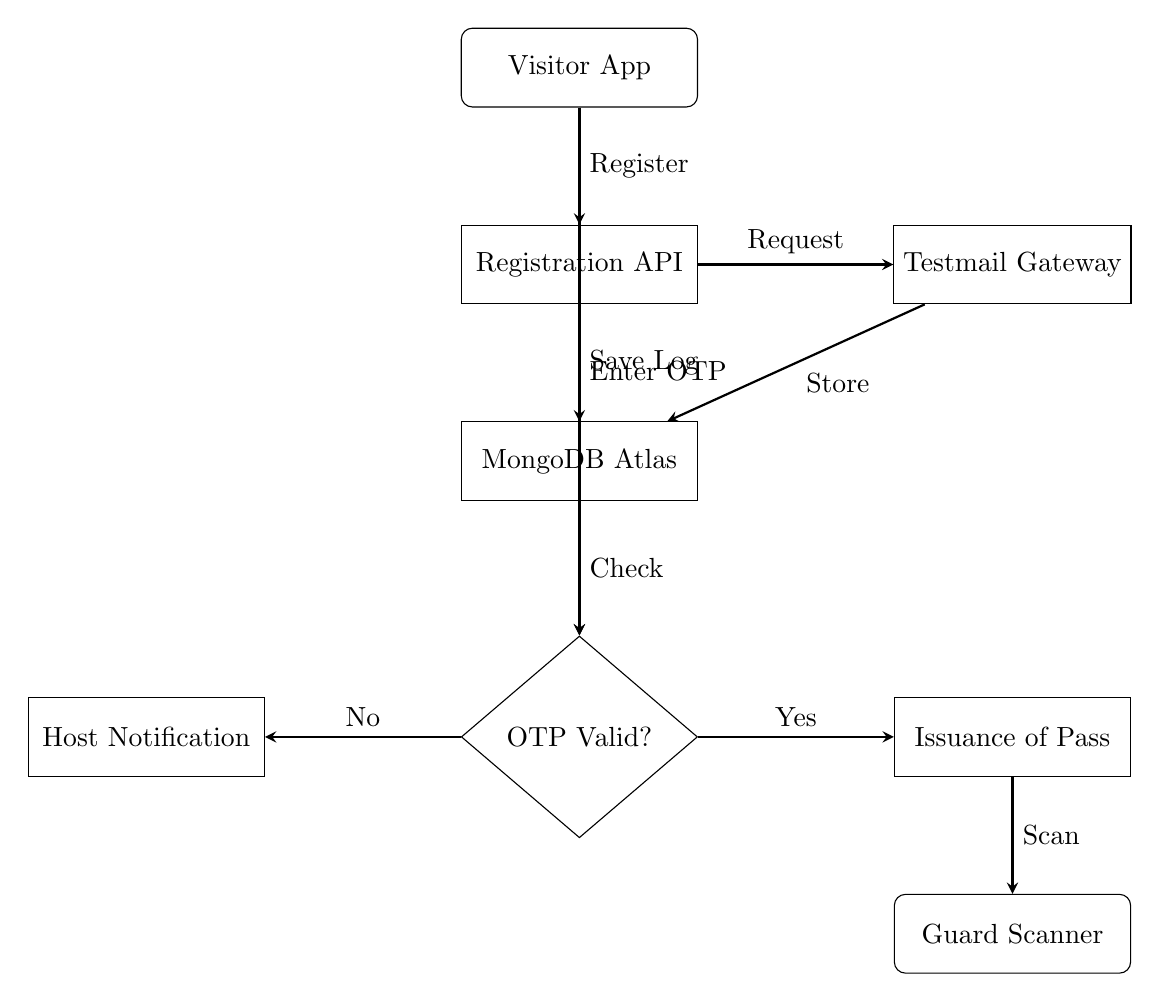
\begin{tikzpicture}[node distance=2.5cm, auto]
    % Nodes
    \node (visitor) [startstop] {Visitor App};
    \node (api) [process, below of=visitor] {Registration API};
    \node (otpgen) [process, right of=api, xshift=3cm] {Testmail Gateway};
    \node (db) [process, below of=api] {MongoDB Atlas};
    \node (verify) [decision, below of=db, yshift=-1cm] {OTP Valid?};
    \node (notify) [process, left of=verify, xshift=-3cm] {Host Notification};
    \node (pass) [process, right of=verify, xshift=3cm] {Issuance of Pass};
    \node (guard) [startstop, below of=pass] {Guard Scanner};

    % Arrows
    \draw [arrow] (visitor) -- node {Register} (api);
    \draw [arrow] (api) -- node {Request} (otpgen);
    \draw [arrow] (otpgen) -- node {Store} (db);
    \draw [arrow] (api) -- node {Save Log} (db);
    \draw [arrow] (visitor) -- node {Enter OTP} (verify);
    \draw [arrow] (db) -- node {Check} (verify);
    \draw [arrow] (verify) -- node[anchor=south] {No} (notify);
    \draw [arrow] (verify) -- node[anchor=south] {Yes} (pass);
    \draw [arrow] (pass) -- node {Scan} (guard);
\end{tikzpicture}
\end{center}

\subsection{System Interaction Diagram}
\begin{center}
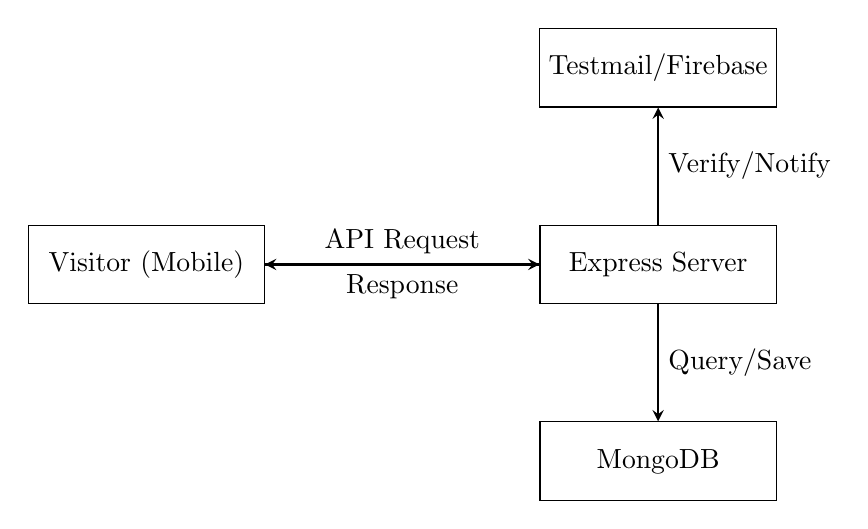
\begin{tikzpicture}[node distance=2.5cm]
    \node (visitor) [process] {Visitor (Mobile)};
    \node (server) [process, right of=visitor, xshift=4cm] {Express Server};
    \node (db) [process, below of=server] {MongoDB};
    \node (ext) [process, above of=server] {Testmail/Firebase};

    \draw [arrow] (visitor) -- node[anchor=south] {API Request} (server);
    \draw [arrow] (server) -- node[anchor=west] {Query/Save} (db);
    \draw [arrow] (server) -- node[anchor=west] {Verify/Notify} (ext);
    \draw [arrow] (server) -- node[anchor=north] {Response} (visitor);
\end{tikzpicture}
\end{center}

\end{document}
